\chapter{Opis implementacji}
\label{Chapter6}

\section{Wstęp}
\label{Chapter61}

{\color{red}Wersja bez redakcji.}

%Wprowadzenie. Struktura tego rozdziału nie jest z góry określona, gdyż mocno zależy to od specyfiki projektu. Generalnie w poszczególnych podrozdziałach każdy powinien opisać swoją część z takiego technicznego punktu widzenia. Piszecie, jak zrealizowaliście poszczególne wymagania, jak to wygląda ,,pod maską'', oczywiście też trzeba przyjąć jakiś poziom szczegółowości. W bardzo szczególnych przypadkach chyba może się zdarzyć, że trzeba będzie załączyć fragment jakiegoś kodu źródłowego czy konfiguracji -- generalnie ma to być opisane w taki sposób, że jako osoba nieznająca systemu siadam i wiem, jak i co zrobiliście. Oczywiście, to moje dywagacje, być może osoby związane z uczelnią zlinczują mnie za ten fragment.

\section{Napotkane problemy i ich rozwiązania}
\label{Chapter62}
%Tu zostanie przeniesiona część treści z wniosków. Wówczas dodane zostaną odpowiednie lub zastosowany zostanie ten sam mechanizm co we Wnioskach.

\section{Użyte technologie}
\label{Chapter63}

\subsection{Moodle}
\emph{Moodle} (roz. \textit{Modular Object-Oriented Dynamic Learning Environment}) -- stanowi podstawę systemu \textit{iQuest}. Jest to popularna (ponad 63 miliony użytkownikiów) platforma e-learningowa o otwartym kodzie źródłowym, napisana w języku \emph{PHP}.Wyboru dokonano ze względu na kilka czynników:
\begin{itemize}
\item{Propozycję Architekta, wynikającą z faktu, iż Moodle posiada już implementację wielu wymaganych w \textit{iQuest} mechanizmów, jak np. konta użytkowników, system ról i uprawnień.}
\item{Oczekiwania Klienta, wynikające z popularności platformy Moodle wśród systemów uczelnianych.}
\item{Modułowość \emph{Moodle}, umożliwiającą pisanie rozszerzeń.}
\end{itemize}

\subsection{PHP}
\emph{PHP} -- platforma \textit{Moodle} jest napisana właśnie w tym języku programowania. Z tego względu, jest to technologia zastosowana w większości rozszerzeń utworzonych przez zespół /textit{iQuest}, korzystających z interfejsów programowania aplikacji tej platformy. Ponadto \emph{PHP} jest jednym z najpopularniejszych języków programowania aplikacji internetowych, posiada doskonalą dokumentację oraz jest cały czas rozwijany.

\subsection{PHPUnit}
Ze względu na fakt, iż programiści \textit{Moodle'a} wykonują testy jednostkowe kodu wykorzystując do tego celu \emph{PHPUnit}, zdecydowano się skorzystać z przygotowanego przez nich oprogramowania. \textit{Moodle} udostępnia dwie klasy do testowania -- \textit{basic\_testcase} i \textit{advanced\_testcase}, przy czym druga wymieniona służy do testów, które wchodzą w interakcję z bazą danych.

\subsection{Selenium}
\emph{Selenium} -- szybko rozwijające się narzędzie do testów akceptacyjnych. Był to naturalny wybór zwłaszcza, że zostało ono przybliżone programistom na zajęciach z Inżynierii Oprogramowania w trakcie toku studiów. Projekt ten składa się m.in. z następującego oprogramowania:
\begin{itemize}
\item{Selenium IDE -- zintegrowane środowisko programistyczne dla skryptów \emph{Selenium} -- zaimplementowane jako rozszerzenie dla przeglądarki internetowej Firefox. Pozwala na: nagrywanie i odtwarzanie sekwencji kroków, wykonywanych podczas pracy z przeglądarką, eksport skryptów do kodu języków programowania (np. \emph{Java}).}
\item{Selenium Client Drivers (\emph{Java}) -- sterownik klienta dla języka Java, pozwalający na wykonywanie skryptów \emph{Selenium} z poziomu języka \emph{Java}},
\item{HtmlUnit Driver} -- Implementacja klasy \emph{WebDriver}, która emuluje zachowanie przeglądarki. Pozwala na uruchamianie skryptów \emph{Selenium} bez korzystania z przeglądarki internetowej.}
\end{itemize}

\subsection{PostgreSQL}
System zarządzania bazą danych \emph{PostgreSQL} został wybrany ze względu na wymaganie pozafunkcjonalne -- pracownicy \emph{Działu Rozwoju Oprogramowania Politechniki Poznańskiej} korzystają z tej właśnie bazy danych. Jest to baza danych o otwartym kodzie źródłowym, zgodna ze standardami, ciągle rozwijana, wysoce konfigurowalna.

\subsection{Eclipse IDE}
\label{Chapter621}

Wybór \emph{Eclipse IDE} jako stosowanego dla projektu \textit{iQuest} zintegrowanego środowiska programistycznego wynika z faktu, iż oprogramowanie to jest dostępne za darmo. Dodatkową zaletą \textit{Eclipse} jest modularność tego rozwiązania, dzięki czemu dostępny jest w nim dodatek \emph{PHP Development Tools}, upraszczający pracę z technologią PHP. Udostępnia m.in. narzędzia do analizy poprawności składniowej pisanego kodu, formatery kodu, wyszukiwanie fraz w wielu plikach, kontekstowe podpowiedzi i nawigację.

\subsection{SVN}
\label{Chapter632}

\emph{Subversion} został wybrany jako podstawowy system kontroli wersji ze względu na wymagania pozafunkcjonalne. Zespół eksploatacji, który docelowo przejmie zarządzanie artefaktami związanymi z projektem, wykorzystuje właśnie \textit{SVN}. Główne funkcjonalności tego systemu to: atomowe publikowanie zmian, historia operacji na plikach (zmiana nazwy, skopiowanie, przeniesienie, modyfikacja, usunięcie), wersjonowanie plików i folderów, łatwy dostęp do informacji o zmianach.

\subsection{Redmine}
\label{Chapter633}

Systemu zarządzania projektami \emph{Redmine} wykorzystywany był od samego początku istnienia projektu. Jest to narzędzie bardzo przydatne w wymianie informacji pomiędzy członkami zespołu, integrujące się m.in. z repozytorium kodu, bazą wiedzy o projekcie, listą zagadnień, forum.  Technologia ta została narzucona, ze względu na sposób organizacji pracy w \textit{Software Development Studio} na Politechnice Poznańskiej.

\subsection{JasperReports}
\label{Chapter634}

Ze względu na wymagania pozafunkcjonalne, zdecydowano się skorzystać z mechanizmów raportowania oferowanych przez \emph{JasperReports}. Jest to najbardziej popularny silnik raportowania o otwartym kodzie źródłowym (wersja Community). Pozwala na generację raportów, których treść jest określona z dokładnością co do piksela. Generowane raporty można eksportować do popularnych formatów dokumentów, np. HTML, PDF, Excel, Word.
\subsection{\textit{JavaScript}}
\label{Chapter63b}

Formularze wymagające częstej interakcji z klientem, np. formularz umożliwiający tworzenie nowej ankiety, oraz funkcje związane z walidacją pól uzupełnianych przez klienta zostały napisane w \textit{JavaScript}. Obsługa strony po stronie klienta jest dla użytkownika niego znacznie wygodniejsza, gdyż nie wymaga częstego przeładowywania całej strony. Dodatkowo, ogranicza to obciążenie łącza zarówno po jego stronie, jak i po stronie serwera, co jest korzystne dla obu stron.

\section{Ogólna struktura projektu}
\label{Chapter64}

{\color{red}Sekcja druga.}

\section{Interfejs}
\label{Chapter65}

Jedną z części pracy było zaprojektowanie graficznego interfejsu użytkownika. Głównym problemem jaki się pojawił, był wybór odpowiedniego narzędzia. Celem jaki postawiono, była maksymalna zgodność projektowanych elementów z różnymi wersjami \emph{Moodle} -- zarówno wcześniejszymi, jak i późniejszymi. Zdecydowano, aby starać się korzystać z gotowych interfejsów programowania aplikacji \emph{(API)} dostarczonych przez \emph{Moodle}, tj. \emph{Page API}, \emph{Form API}, oraz \emph{Access API}. Wszystkie interfejsy są napisane przy użyciu języka PHP -- są wykonywane po stronie serwera. Konieczne okazało się też wykonanie niektórych skryptów po stronie klienta. Dlatego w projekcie wykorzystano również język skryptowy \emph{Java Script}.

\section{Logika (back-end)}
\label{Chapter66}

Jednym z zadań w ramach pracy było zaprogramowanie odpowiedniej logiki biznesowej rozwiązującej zadania stawiane przed zaprojektowanym systemem. Najważniejszym zadaniem z perspektywy back-end'u jest interakcja z bazą danych. Poza tym system posiada: procesor zadań wykonywanych w tle oparty na \emph{cron}; moduły odpowiadające za komunikację z systemami uczelanianymi \emph{ePoczta} i \emph{eDziekanat}; moduł logowania zdarzeń. W trakcie implementacji zdecydowano się nie tworzyć osobnego mechanizmu do przechowywania ustawień w bazie danych i skorzystaliśmy z istniejącego już w \emph{Moodle}. Jednym z wymagań pozafunkcjonalnych było wykorzystanie bazy danych \emph{PostgreSQL}. Platforma \emph{Moodle} korzysta z mechanizmu \emph{XMLDB}, co pozwala na ominięcie wielu problemów pojawiających się przy migracjach pomiędzy różnymi systemami baz danych. Niestety kosztem wykorzystania tego mechanizmu jest konieczność pracy z interfejsami programowania aplikacji dostarczanym przez platformę \emph{Moodle} -- \emph{Data manipulation API}. Na diagramie poniżej znajdują się także klasy przechowujące stałe: (\emph{tables}, \emph{settings}.\\

\begin{figure}[H]
\begin{center}
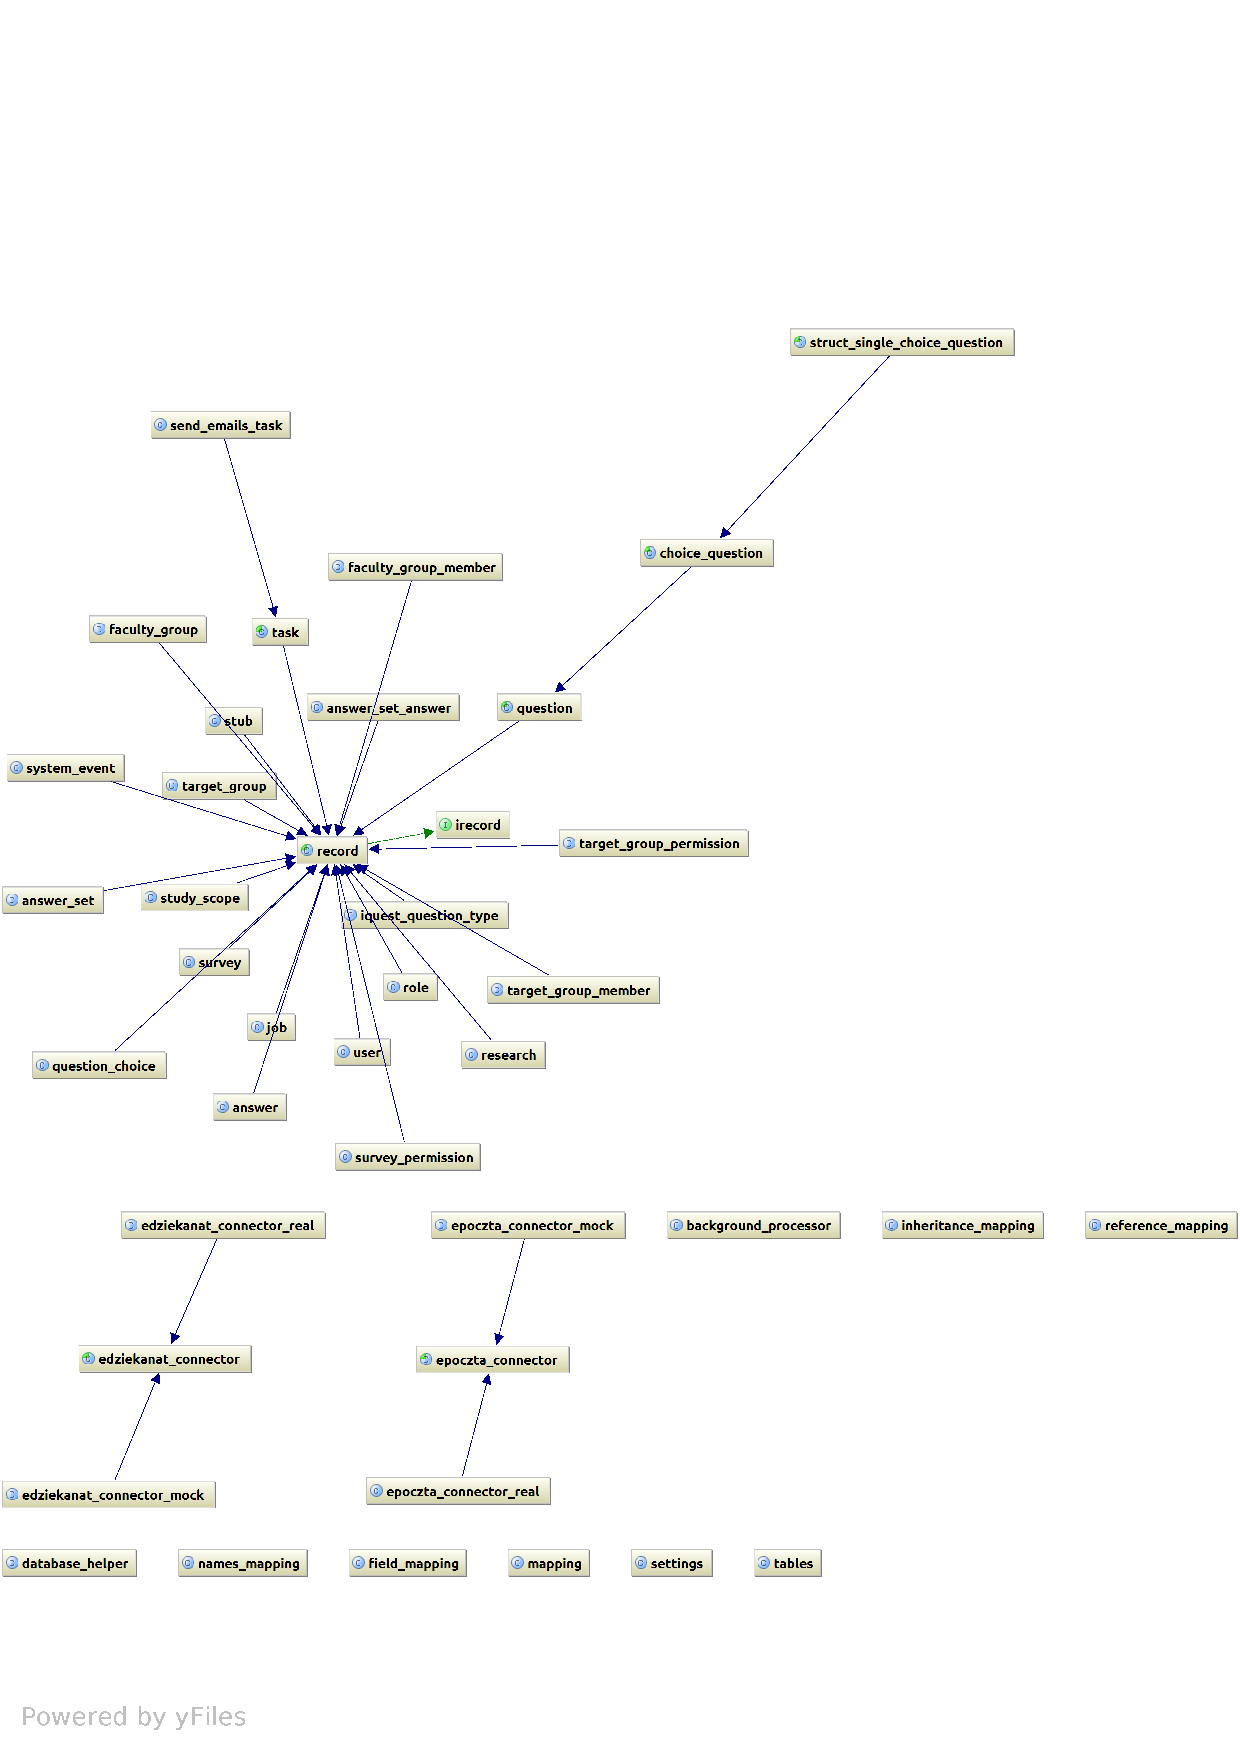
\includegraphics[width=0.9\textwidth]{figures/lw/backend.pdf} 
\end{center}
\caption{Struktura back-end'u}
\label{fig:back-end}
\end{figure}

\subsection{Raporty}
Raporty wykonano korzystając z platformy JasperReports, wykorzystując następujące produkty firmy \emph{Jaspersoft}:

\begin{itemize}
\item \emph{JasperReports Server} (wersja 5.0) -- serwer usług raportowania, na którym przechowywane są przygotowane przez zespół artefakty, w celu umożliwienia generacji raportu osobom dysponującym odpowiednimi uprawnieniami. Wykorzystano następujące funkcjonalności: definiowania źródła danych, raportu, ładowania plików z projektem raportu, zasobami oraz z generacji raportu.
\item \emph{Jaspersoft Studio} (wersja 1.3.2) -- bazowane na Eclipse narzędzie do projektowania raportów. Posłużyło zespołowi do przygotowania projektów raportów w formacie \emph{JRXML}.
\end{itemize}

Kody źródłowe pakietu \emph{JasperReports} są pisane w języku Java. Źródłem danych dla raportu, jest przygotowana przez zespół implementacja interfejsu \emph{ReportDataSourceService} z \emph{API JasperServer}. Źródło danych łączy się z udostępnianymi przez wskazaną instancję systemu \emph{iQuest} usługami zdalnymi, z których otrzymuje informacje o przeprowadzanych badaniach poprzez protokół SOAP. Struktura raportu zależy od typu pytania (otwarte/zamknięte). W przypadku pytań otwartych prezentowana jest lista odpowiedzi. Dla pytań zamkniętych na podstawie pobranych danych generowane są statystyki, które przekazywane są do podraportu w postaci obiektu klasy \emph{JRBeanCollectionDataSource}. W generacji statystyk z danych badań wykorzystano bibliotekę \emph{JoSQL}. Definicja projektu raportu składa się z czterech plików, odpowiadających trzem kolejnych poziomom:
\begin{enumerate}
\item \emph{researches.jrxml} -- raport główny dla badań,
\item \emph{questions.jrxml} -- podraport pytań,
\item \emph{answers\_closed.jrxml} oraz \emph{answers\_open.jrxml} -- podraporty odpowiedzi. zamkniętych i otwartych.
\end{enumerate}
Do generacji namiastek obiektów zdalnych (ang. \definicja{stub}) wykorzystano Apache Axis. Wygenerowane klasy dostosowano tak, by akceptowały obiekty z zadanej instancji \emph{iQuest} oraz dla zmiennej przestrzeni nazw (ang. \emph{namespace}).\\

W trakcie generacji \emph{stub'ów} okazało się, iż definicja usług dla protokołu \emph{SOAP} w języku \emph{WSDL} (\emph{Web Service Description Language}) generowana przez \emph{Moodle} jest niepoprawna. Skorzystano zatem z poprawionej wersji z zewnętrznego źródła (\url{https://github.com/ghigio/moodle-webservice_soapfda}).\\

Dostęp do usług zdalnych definiowanych w \emph{Moodle} zabezpieczono korzystając z mechanizmu generacji tokenu dla wybranego użytkownika. Użytkownik, który z poziomu serwera \emph{Jasper Server} zamierza wygenerować raport, musi znać adres naszego systemu oraz posiadać token dostępu do usługi.

\subsection{Moduły uwierzytelniania}
Korzystając z mechanizmów rozszerzeń \emph{Moodle} zaimplementowano dwa moduły uwierzytelniania, tj.:
\begin{itemize}
\item \emph{eKontoAuthenticationPlugin} -- integruje logowanie przez \emph{eKonto} z naszym systemem,
\item \emph{emailgraduate} -- pozwala absolwentom uczelni na rejestrację z użyciem adresu e-mail.
\end{itemize}

W celu spełnienia wymagań Działu Rozwoju Oprogramowania Politechniki Poznańskiej odnośnie wygaszania sesji użytkownika \emph{eKonto} po zadanym czasie (e.g. 15 min.) zmodyfikowano pliki źródłowe \emph{Moodle}, gdyż dla kodu odnoszącego się do sesji użytkownika \emph{Moodle} nie została przewidziana możliwość rejestracji rozszerzeń. Relacja \emph{user} została rozszerzona o opcjonalne pola związane z \emph{eKonto}, jako że kod odpowiedzialny za manipulację schematem bazy danych nie jest wykonywany podczas instalacji modułu uwierzytelniania, umieszczono go w osobnym module (\emph{ekontodb}). \emph{eKontoAuthenticationPlugin} może być instalowany bez konieczności instalacji \emph{iSurvey}. Podczas jego implementacji korzystaliśmy z dokumentu \emph{Centralne uwierzytelnianie i wymiana danych. Wersja 1.2 (2010.07.06)}.\\

Podczas rejestracji z użyciem naszych modułów użytkownik jest przydzielany do grupy docelowej ,,Absolwenci'', nadawana jest mu też rola respondenta w kontekście \emph{kursu iQuest}. Utworzenie modułu wiąże się z przygotowaniem klasy dziedziczącej z \emph{auth\_plugin\_base}, formularza ustawień, pliku lokalizacji oraz wersji.

\subsection{Moduły dla serwisów zewnętrznych}
\begin{itemize}
\item \emph{ePocztaConnector} -- służy do wysyłania e-maili z serwera Politechniki Poznańskiej,
\item \emph{eDziekanatConnector} -- pobiera i aktualizuje lokalne informacje o grupach dziekańskich, zakresach tematycznych tychże grup oraz ich studentach.
\end{itemize}

\emph{Dział Rozwoju Oprogramowania} udostępnia klienty \emph{eUsług} dla różnych języków, w tym dla \emph{PHP}. Komunikacja z usługami zdalnymi uczelni odbywa się poprzez protokół SOAP. Wyżej wymienione moduły zaimplementowano z wykorzystaniem fabryki obiektów, która w zależności od trybu (testowy/produkcyjny) zwraca obiekt odpowiedniej klasy. Zadania związane z oba modułami są zlecane procesorowi zadań w tle.

%to poleci gdzieś indziej.
%\begin{landscape}

%\begin{figure}[!th]
%\centering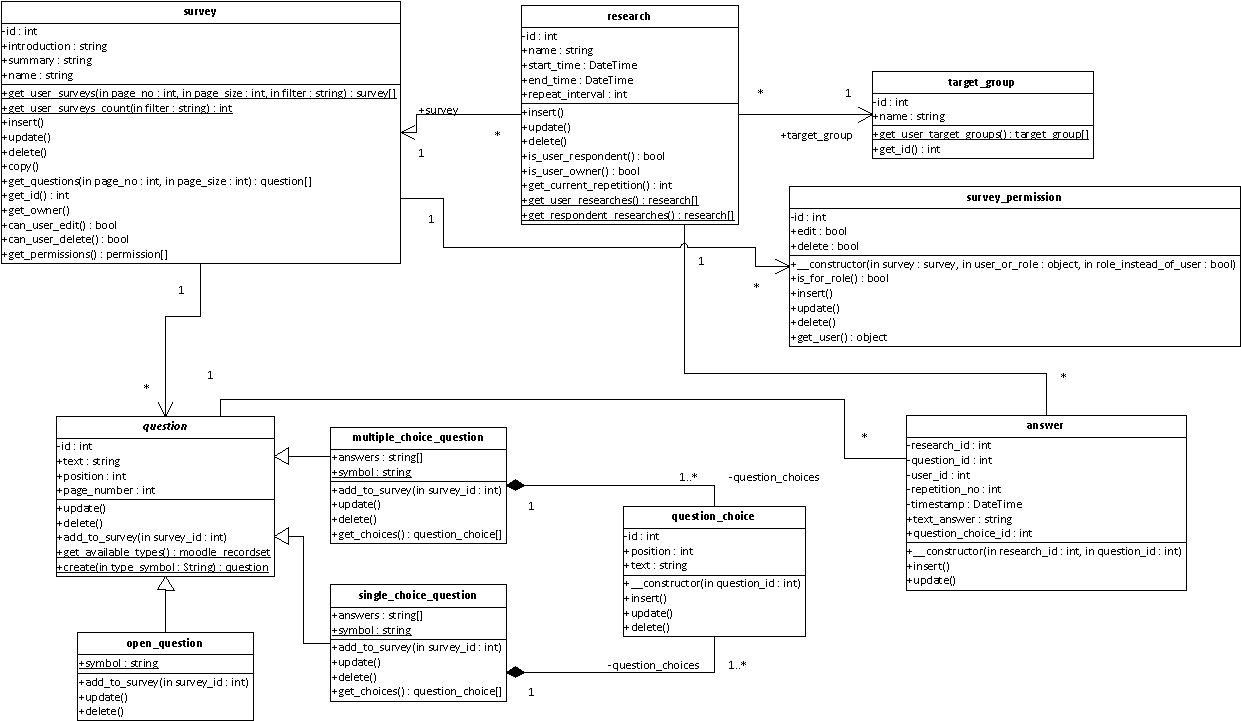
\includegraphics[width=1.25\textheight]{figures/Survey_Creator_Survey_Runner.png}
%\caption{Backend -- moduły Survey Creator i Survey Runner}\label{rys:iquest-backend}
%\end{figure}

%\begin{figure}[!th]
%\centering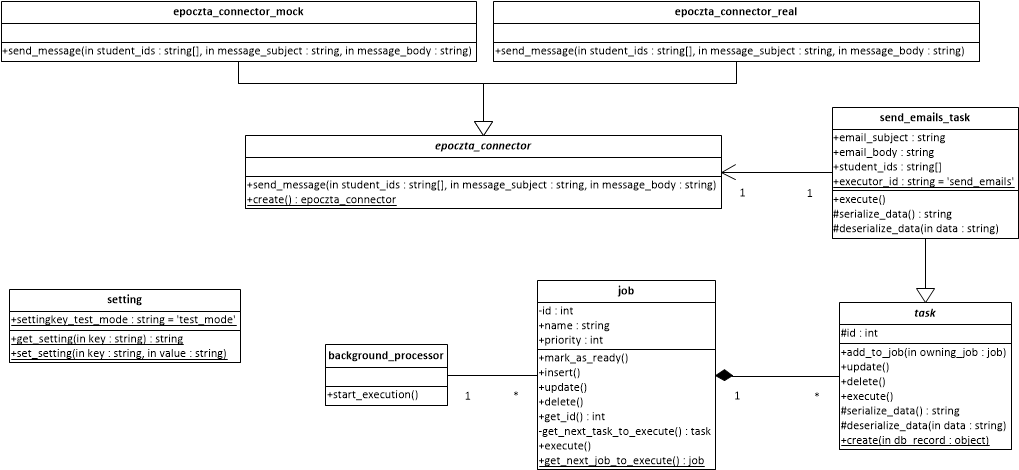
\includegraphics[width=1.25\textheight]{figures/ePoczta_Connector_Background_Task_Scheduler_and_Executor.png}
%\caption{Backend -- moduły ePoczta Connector i Background Task Scheduler and Executor}\label{rys:iquest-backend2}
%\end{figure}

%\end{landscape}

\section{Powiązanie back-endu z interfejsem}
\label{Chapter67}

%brak treści?